% !TeX encoding = utf8
\documentclass[aspectratio=169]{beamer}

\usepackage[english]{babel}
\usepackage{amsmath}
\usepackage{amssymb}
%\usepackage{mathpazo}
%\usepackage{palatino}
%\usefonttheme{professionalfonts}
%\renewcommand\familydefault{\rmdefault}
\usefonttheme[onlymath]{serif}

\DeclareMathOperator*{\E}{\mathbf{E}}
\DeclareMathOperator*{\Prob}{\mathbf{P}}
\newcommand{\A}{\mathbf{A}}
\newcommand{\Pro}{\mathbf{P}}
\newcommand{\xx}{\mathbf{x}}
\newcommand{\bb}{\mathbf{b}}
\newcommand{\ee}{\mathbf{e}}
\newcommand{\pp}{\mathbf{p}}
\newcommand\inner[2]{\langle #1, #2 \rangle }
\newcommand{\R}{\mathbb{R}}

\DeclareMathOperator*{\argmax}{arg\,max}
\DeclareMathOperator*{\argmin}{arg\,min}

\addtobeamertemplate{navigation symbols}{}{%
	\usebeamerfont{footline}%
	\usebeamercolor[fg]{footline}%
	\hspace{1em}%
	\insertframenumber/\inserttotalframenumber
}

\title{Hands on Machine Learning}
\subtitle{Chater 2}
\author{\href{mailto:zoennchen.benedikt@hm.edu}{\textbf{Benedikt Z\"onnchen}}} 
\date{\today}
%\setdefaultlanguage[spelling=new]{german}

\begin{document}
	
	\begin{frame}
		\titlepage
	\end{frame}

	\begin{frame}
		\begin{block}{Problem}
			Given 8 attributes (longitude, latitude, house age, rooms, bedrooms, population, households, income), we want to predict the (mean) \textit{house value}.
		\end{block}
	\end{frame}

	\begin{frame}
		\frametitle{Data inspection}
		\begin{figure}
			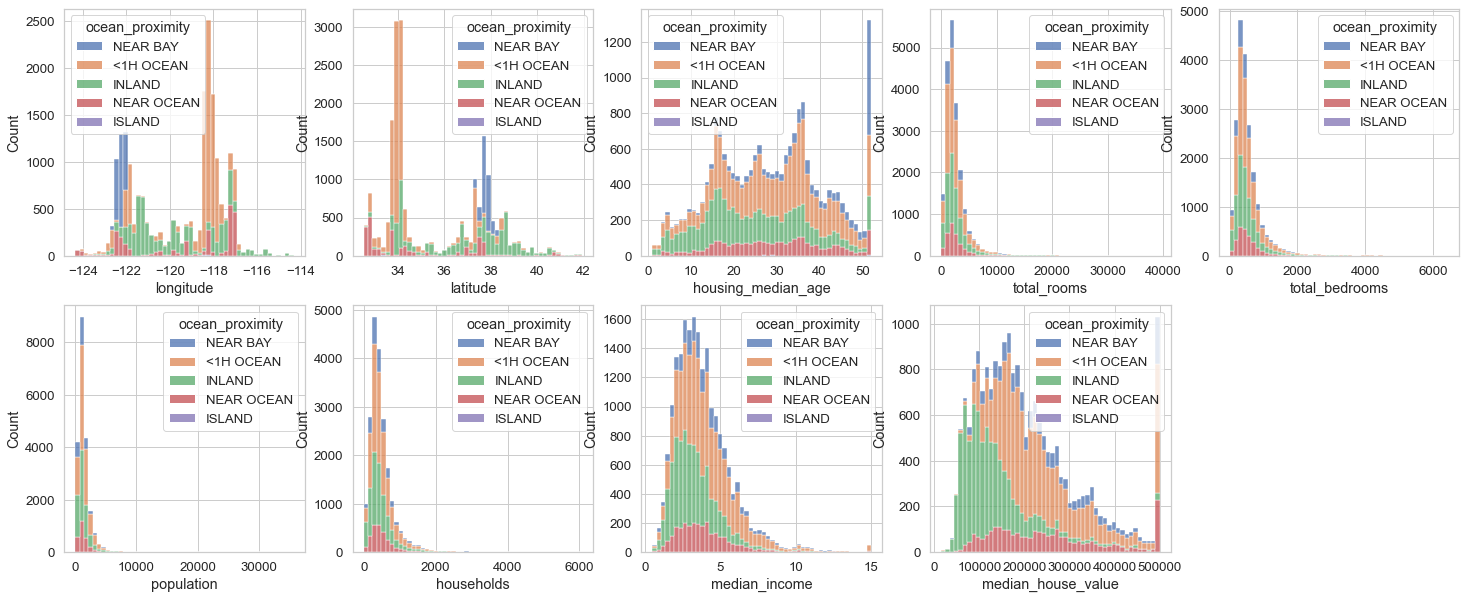
\includegraphics[width=\textwidth]{./../plots/histos.png}
		\end{figure}
	\end{frame}

	\begin{frame}
		\frametitle{Data inspection}
		Strong correlation between \textit{rooms}, \textit{bedrooms} \textit{households} and \textit{population}:
		\begin{figure}
			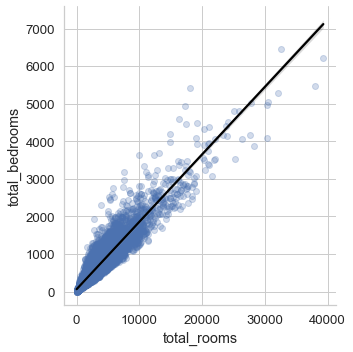
\includegraphics[width=0.30\textwidth]{./../plots/rooms_bedrooms.png}
			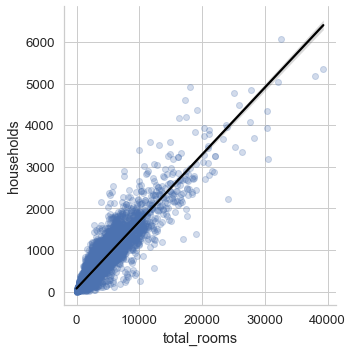
\includegraphics[width=0.30\textwidth]{./../plots/rooms_households.png}
			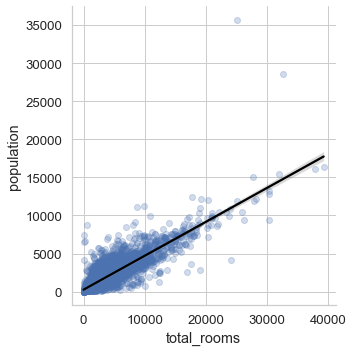
\includegraphics[width=0.30\textwidth]{./../plots/rooms_population.png}
		\end{figure}
	\end{frame}

	\begin{frame}
		\frametitle{Data inspection}
		How does the \textit{house value} change with \textit{ocean proximity} (discrete category)?
		\begin{figure}
			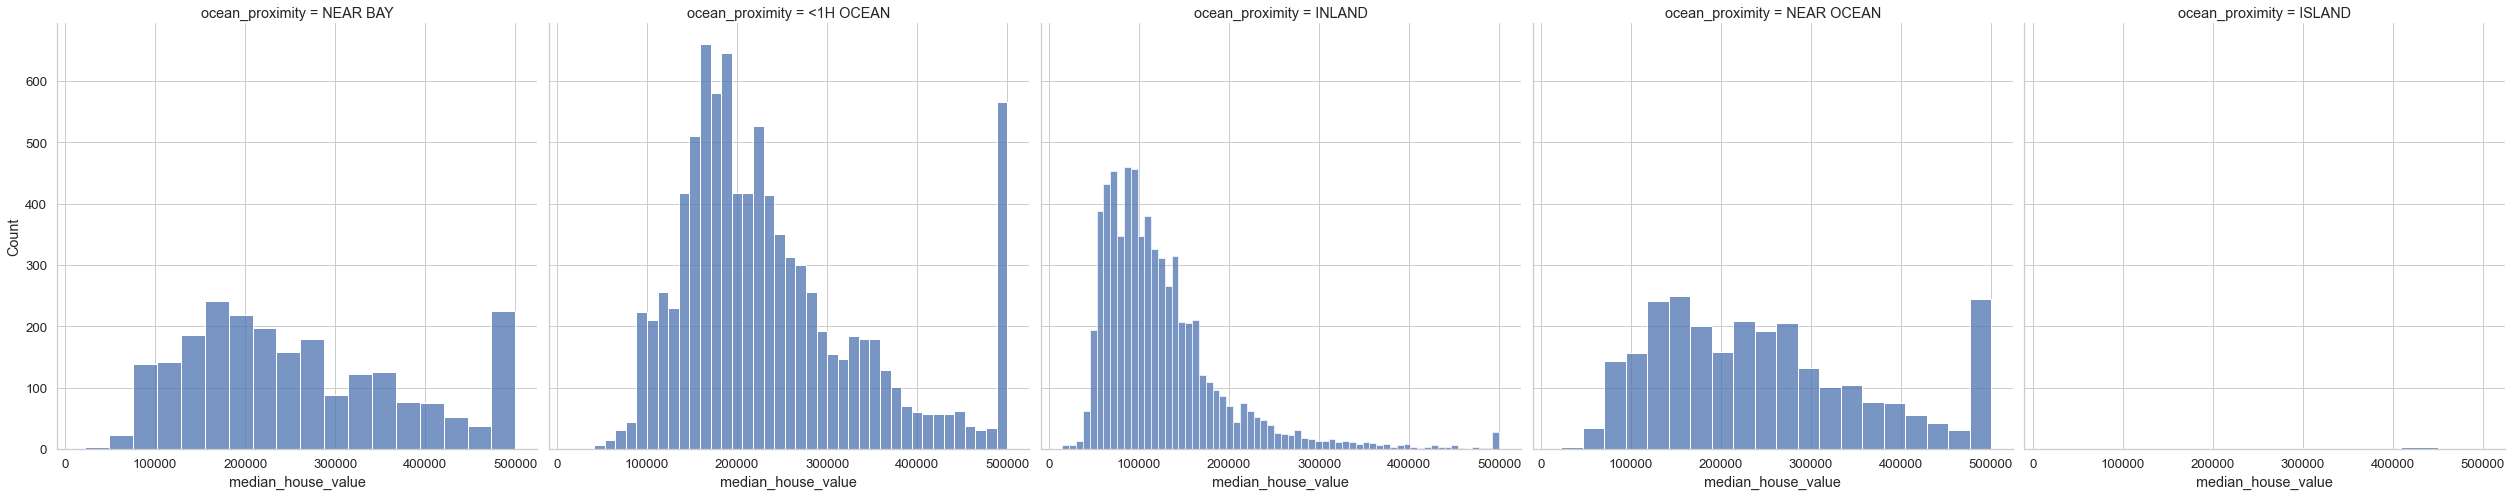
\includegraphics[width=\textwidth]{./../plots/house_value_ocean.png}
		\end{figure}
		\begin{itemize}
			\item \textit{near bay} and \textit{near ocean} look similar
			\item \textit{inland} house values are more lean towards the lower end
			\item there are some very expensive houses hidden in the data
		\end{itemize}
	\end{frame}
	
		\begin{frame}
		\frametitle{Data inspection}
		\begin{figure}
			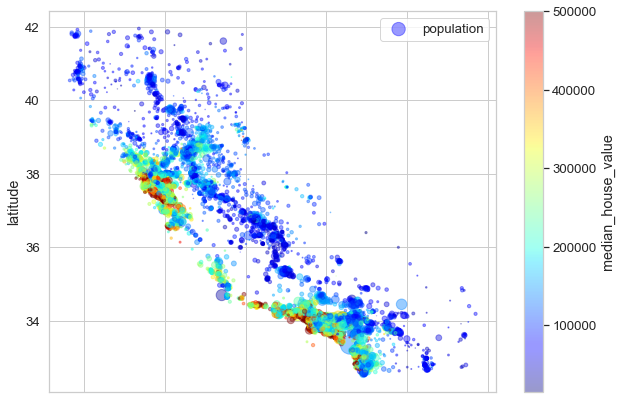
\includegraphics[width=0.7\textwidth]{./../plots/heatmap.png}
		\end{figure}
	\end{frame}
	
	\begin{frame}
		\frametitle{Data inspection}
		\begin{columns}
			\begin{column}{0.5\textwidth}
				\begin{itemize}
					\item \textit{income} and \textit{house value} are correlated
					\item everything else is not really correlated with the \textit{house value}
				\end{itemize}
			\end{column}
			\begin{column}{0.5\textwidth}
				\begin{figure}
					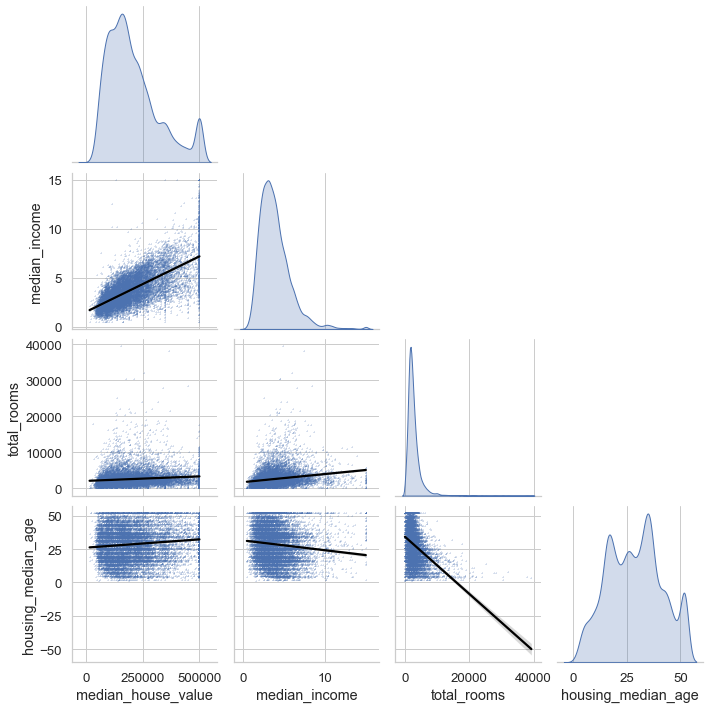
\includegraphics[width=\textwidth]{./../plots/corrolations.png}
				\end{figure}
			\end{column}
		\end{columns}
	\end{frame}

	\begin{frame}
		\frametitle{Machine learning pipeline}
		\textbf{Preparation}:
		\begin{enumerate}
			\item Preparation
			\item download the data
			\item load the data
			\item inspect the data
			\item add \textit{income category} to split the data effectively
			\item split the data into \textit{training set} and \textit{test set} (0.8/0.2)
			\item split the \textit{training set} into \textit{label} and \textit{remaining data}
			\item \textbf{data cleaning}: deal with missing data (fill, drop row, or drop attribute)
			\item convert categories into numbers
			\item add combined attributes
			\item \textbf{feature scaling}: \textit{normalization} or \textit{standardization}
		\end{enumerate}
	\end{frame}

	\begin{frame}
		\frametitle{Machine learning pipeline}
		\textbf{Model creation}:
		\begin{enumerate}
			\item select and train a (or multiple) model(s) (\textbf{use cross-validation})
			\item select your shortlist of promising models
			\item fine-tune your model: 
			\begin{itemize}
				\item hyperparameter optimization: \textit{random walk}, \textit{grid search} (\textbf{use cross-validation})
				\item ensemble methods: combine your best models
				\item feature manipulation: drop non-influential features
			\end{itemize}
			\item evaluate your result on the \textit{test set}
		\end{enumerate}
		\textbf{Build your system}
	\end{frame}

	\begin{frame}
		\frametitle{Pitfalls/remarks}
		Correlation captures only \textbf{linear} relations:
		\begin{figure}
			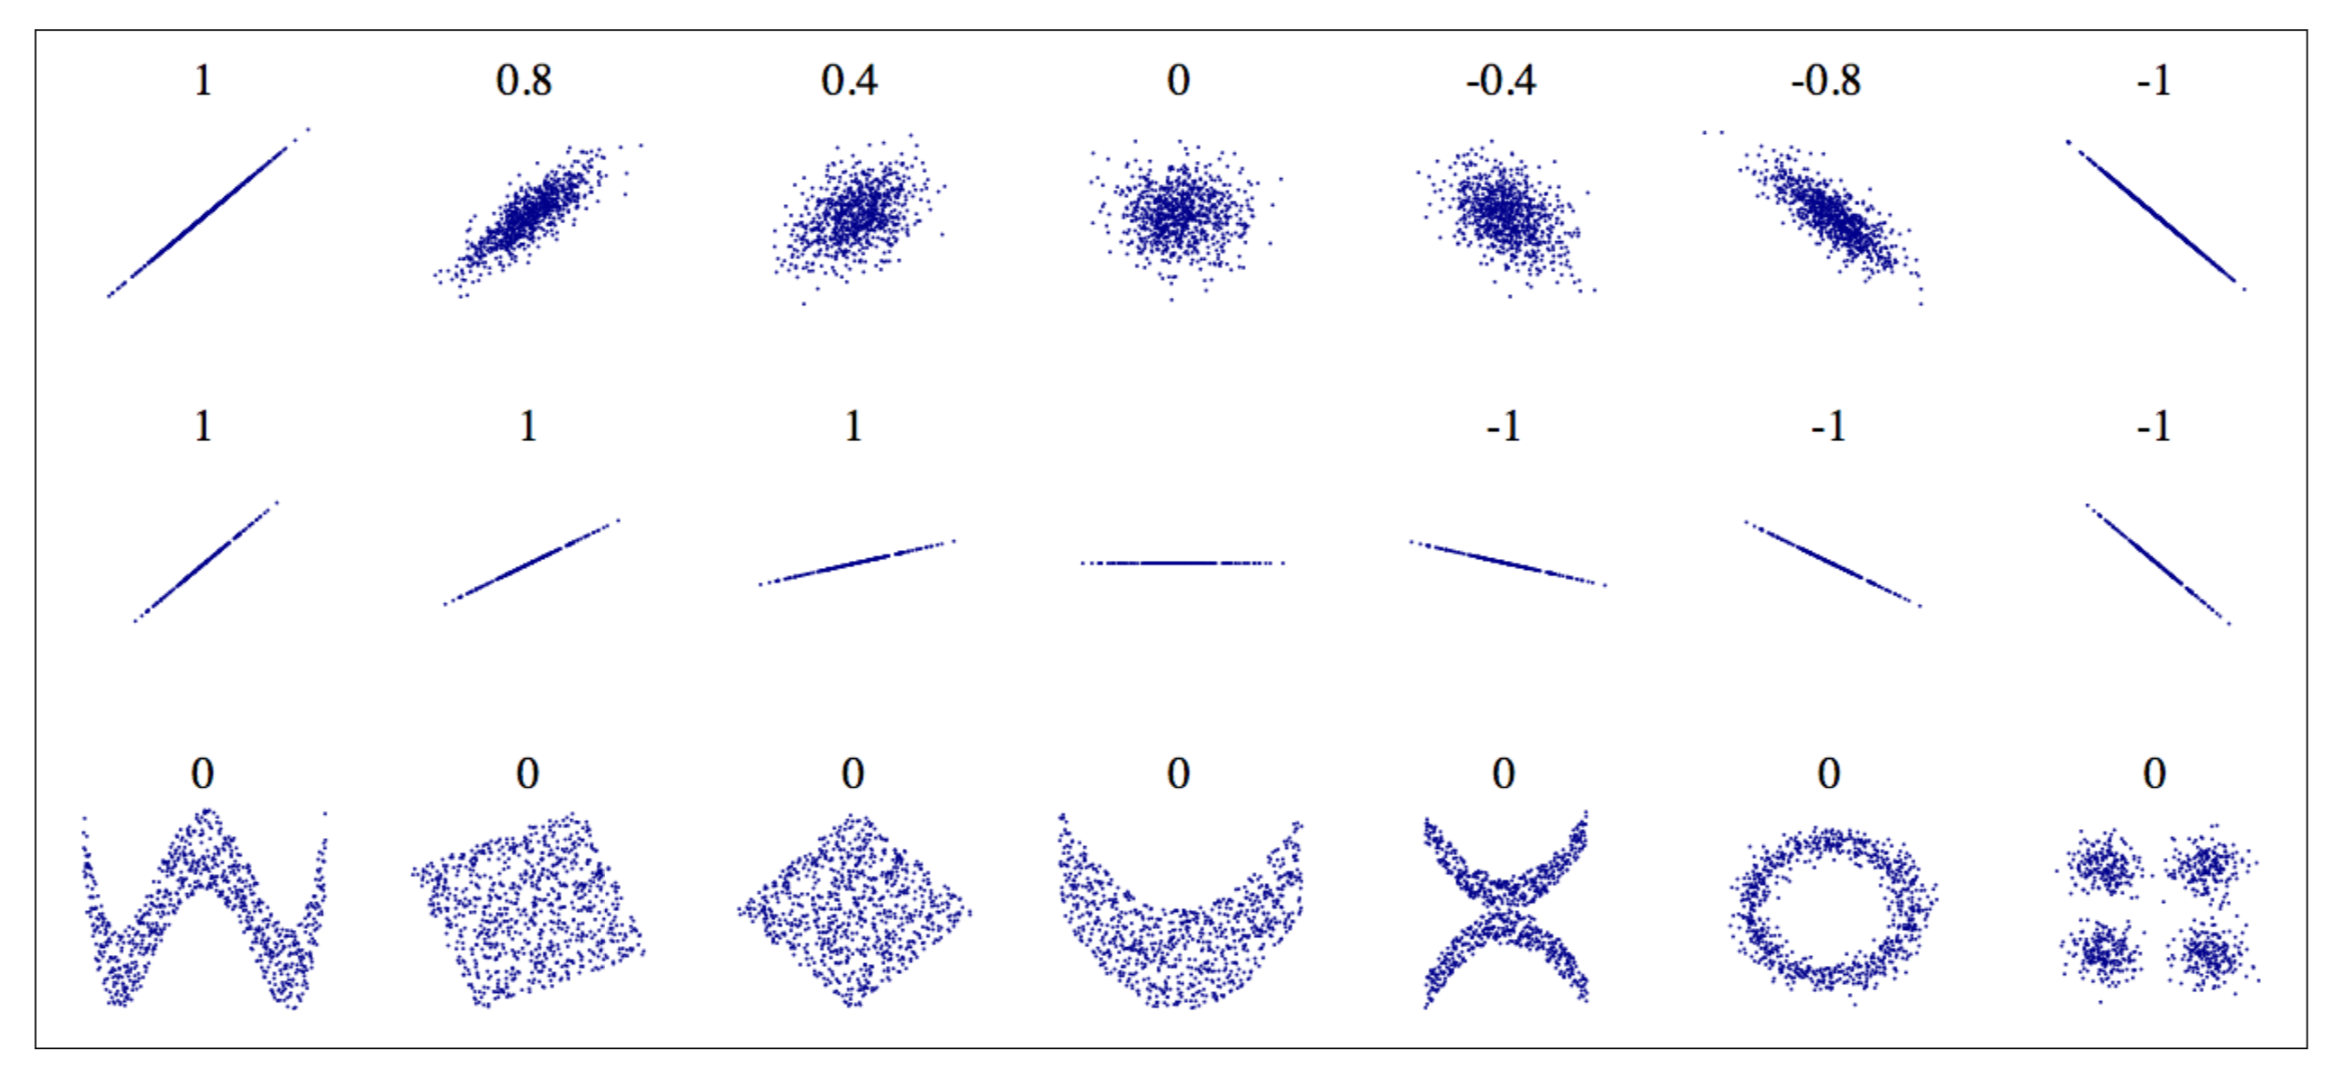
\includegraphics[width=\textwidth]{./../figs/correlations.png}
		\end{figure}
	\end{frame}
	
	\begin{frame}
		\frametitle{Pitfalls/remarks}
		Be careful if you use your \textit{test set}:
		\begin{itemize}
			\item if you have not a lot of data, group your data before splitting
			\item use cross-validation
			\item adapting the model after evaluation (using the \textit{test set}) leads to \textit{overfitting}
		\end{itemize}
	\end{frame}

	\begin{frame}
		\frametitle{Terms}
		\begin{block}{Random variable (informal)}
		A random variable is a measurable \textbf{function} from a probability space (set of possible outcomes) $\Omega$ into a measurement space $E$.
		\end{block}
		\vspace{0.5cm}
		The probability $\Prob$ that the random variable $X$ takes on a value in $S \subseteq E$ is noted as
		\begin{equation*}
			\Prob(X \in S) = \Prob(\left\{ \omega \in \Omega : X(\omega) \in S \right\})
		\end{equation*}
		The probability $\Prob$ that the random variable $X$ takes on a value in $x \in E$ is noted as
		\begin{equation*}
			\Prob(X = x) = \Prob(\left\{ \omega \in \Omega : X(\omega) = x \right\})
		\end{equation*}
	\end{frame}

		\begin{frame}
		\frametitle{Terms}
		\begin{block}{Expected value (finite)}
			Let $X$ be a \textit{random variables} with a \textbf{finite} list of values $x_1, \ldots, x_k$ than the \textit{expected value} $\mu_X$ of $X$ is defined by 
			\begin{equation}
				\mu_X = \E[X] = \sum\limits_{i=1}^k x_i \cdot \Prob(X = x_i)
			\end{equation}
		\end{block}
		The expected value is a weighted average of the $x_i$ values.
	\end{frame}

		\begin{frame}
		\frametitle{Terms}
		\begin{block}{Standard deviation}
			Let $X$ be a \textit{random variables} than the \textit{standard deviation} $\sigma_X$ of $X$ is defined by 
		\begin{equation}
			\sigma_X = \sqrt{\E[(X- \mu_X)^2]} =  \sqrt{\E[(X- \E[X])^2]}
		\end{equation}
		\end{block}
		The standard deviation is the square root of the \textit{variance}.
	\end{frame}

	\begin{frame}
		\frametitle{Terms}
		\begin{block}{Correlation}
			Let $X, Y$ be two random variables with \textit{expected values} $\mu_X, \mu_Y$ and \textit{standard deviations} $\sigma_X, \sigma_Y$ than the correlation coefficient is defined by
			\begin{equation}
				\rho_{X,Y} = \text{corr}(X,Y) = \frac{\text{cov}(X,Y)}{\sigma_X \cdot \sigma_Y} = \frac{\E[(X-\mu_X) \cdot (Y - \mu_Y)]}{\sigma_X \cdot \sigma_Y}.
			\end{equation}
		\end{block}
		where $\E[X]$ is the expected value of $X$, i.e., $\mu_X = \E[X]$ and $\mu_Y = \E[Y]$.
	\end{frame}

	\begin{frame}
		\frametitle{Terms}
		\begin{block}{Cross-validation}
			Let $T$ be our data points with $|T| = N$. Let $k < N$ than we $k$ subsets:
			\begin{equation*}
				T_1, \ldots, T_k \subset T
			\end{equation*}
			Than we \textit{train} and \textit{validate} $k$ models by using 
			\begin{equation*}
				\{T_1, \ldots, T_k\} \setminus \{T_i\}
			\end{equation*}
			as \textit{training set} and
			\begin{equation*}
				T_i
			\end{equation*}
			as \textit{test set} for $i \in \{1, \ldots, k\}$.
		\end{block}
	\end{frame}

	\begin{frame}
		\frametitle{Terms}
		\begin{block}{$k$-fold cross-validation}
			Use a partition, that is,
			\begin{equation*}
				\bigcup\limits_{i = 1}^k T_i = T \text{ and } 	i \neq j \Rightarrow T_i \cap T_j = \emptyset 
			\end{equation*}
			holds.
			\begin{figure}
				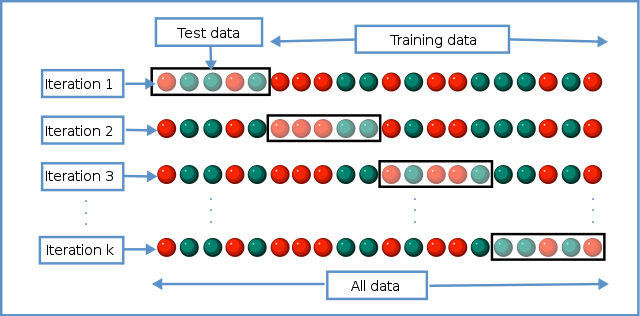
\includegraphics[width=0.55\textwidth]{./../figs/cross-validation.png}
			\end{figure}
		\end{block}
	\end{frame}

		\begin{frame}
		\frametitle{Terms}
		\begin{block}{Normalization (scaling)}
			Shift and rescale (\textbf{linear transformation}) values such that they all lie in $[0;1]$:
			\begin{equation}
				f(x) = \frac{x - x_\text{min}}{x_\text{max} - x_\text{min}} 
			\end{equation}
			Many algorithms expect \textit{normalized} values.
		\end{block}
	\end{frame}

		\begin{frame}
		\frametitle{Terms}
		\begin{block}{Standardization (scaling)}
			Shift by the mean value and scale by the standard deviation (\textbf{linear transformation}):
			\begin{equation}
				y = f(x) = \frac{x - \mu_X}{\sigma_X} 
			\end{equation}
			The resulting distribution has unit variance and is centered around zero.
			The scaling is less affected by \textit{outliers}.
		\end{block}
	\end{frame}
\end{document}